%! TEX ROOT = ./main.tex
\section{The Solution Outline}

%We use a combination of methods to solve the problem.
%First, we quickly obtain a \emph{global} controller $C^\times$ for the product control system $\Sigma^\times_\tau$ using the fast and scalable tool, called ALTRO.
%In principle, any other fast method, suitable for large systems, can be used for this stage.
%ALTRO does not support disturbances, and so we ignore it in this stage.
%ALTRO give us a rough open-loop controller $C^\times$ for the product system $\Sigma^\times$.
%Second, thanks to the decentralized control architecture, we can easily decompose $C^\times$ into nominal local controllers $\set{C^i_\nom}$ for the individual robots.
%The set of controllers $\set{C^i_\nom}$ are actually used as a set of initial guesses for the 
%In the lower level, we rigorously obtain \emph{local} controllers $\set{C^i}$ using ABCD, to track---with formal guarantees against the disturbances---the intended nominal trajectories.
%
%In the lower level, we use ABCD to synthesize a controller that will track the nominal trajectory

We summarize our approach for algorithmic solution of the posed problem in Alg.~\ref{alg:main}.

\begin{algorithm}
\caption{Multi-robot Controller Synthesis}
\label{alg:main}
\begin{enumerate}
	\item For every $i$, let $\Sigma_{\tau,\nom}^i = (X^i,x_\init^i,U^i,\set{0},f^i,Y,h^i)$ be the respective \emph{nominal} control system that ignores the disturbances.
			Compute the product control system $\Sigma^\times_{\tau,\nom}$ of $\set{\Sigma^i_{\tau,\nom}}$. 
			Let $\varepsilon\in \mathbb{R}^n_{>0}$ be a robustness margin; a discussion on $\varepsilon$ follows subsequently.
			Use ALTRO to compute an open-loop controller $C^\times_{\nom}$ for $\Sigma^\times_{\tau,\nom}$ so that $C^\times_\nom\triangleright\Sigma_{\tau,\nom}^{\times}$ realizes  $\Phi_\varepsilon$.
			Let $T$ be the time horizon when $\Phi_\varepsilon$ has been fulfilled for the first time. \label{step:altro}
	\item Decompose $C^\times_\nom$ into \emph{local} open-loop controllers $\set{C^i_\nom}$ for the set of sampled-time abstractions $\set{\Sigma^i_{\tau,\nom}}$.
			The decomposition is straightforward since $C^\times_\nom$ is open-loop.
	\item For every $i$, find the unique nominal open-loop trajectory $\rho^i=(x_{0,\nom}^i,\ldots,x_{T,\nom}^i)$ of length $T$ of $C^i_\nom\triangleright \Sigma_{\tau,\nom}^i$---unique, because there is no disturbance. \label{step:abcd}
			Let $\varepsilon^i\in \mathbb{R}^{n_i}_{>0}$ be the projection of $\varepsilon$ to the state dimensions of $\Sigma_{\tau}^i$.
			Use ABCD to find a closed loop controller $C^i$ for $\Sigma_{\tau}^i$ so that $C^i\parallel \Sigma_\tau^i$ \emph{tracks} the nominal trajectory $\rho^i$, i.e., $C^i\parallel \Sigma_\tau^i$ satisfies the following specification:
			\begin{align}
				\label{eq:ltl_spec}
				\Phi_{\track}^i\coloneqq \ball_{\varepsilon^i}(x_{0,\nom}^i) \wedge \bigwedge_{k\in [1;T]} \bigcirc^t \ball_{\varepsilon^i}(x_{k,\nom}^i),
			\end{align}
			where $\bigcirc^t$ represents the juxtaposition of $t$ consecutive ``$\bigcirc$'' operators.
\end{enumerate}
\end{algorithm}

It can be observed that if every  $C^i\parallel \Sigma_\tau^i$ can realize $\Phi_\track^i$, then because the simultaneous satisfaction of $\rho^i$-s for every $i$ implies satisfaction of $\Phi_\varepsilon$ by design, and because $\Phi_\varepsilon$ is an $\varepsilon$-robust version of $\Phi$, hence it follows that $\set{C^i}_{i\in [1;N]}\parallel \set{\Sigma_\tau^i}_{i\in [1;N]}$ will realize $\Phi$.

%We did not yet mention the role of the robustness margin $\varepsilon$.
%Essentially, $\varepsilon$ accounts for the possible tracking error of the ABCD-generated controller in Step~\ref{step:abcd} while tracking the nominal trajectory.
%Because ALTRO ignores the disturbances, hence a positive tracking error is inevitable.
%For this reason, if we choose $\varepsilon$ too small, then it will be more difficult for ABCD to find a controller against the worst case disturbances, and we might not be able to obtain a controller in Step~\ref{step:abcd} in the end.
%On the other hand, if we choose $\varepsilon$ too large, then it will be more difficult for ALTRO to find a nominal open-loop controller in the first place.
%So ideally, in Step~\ref{step:altro}, we should maximize $\varepsilon$ so that an open-loop controller can be obtained by ALTRO for $\Phi_\varepsilon$.
%For this work, we did not implement this step in an algorithmic manner, and relied on the judgment of the system designer for choosing a suitable $\varepsilon$.

\begin{remark}
	Unfortunately, ALTRO only supports bounded horizon control problem.
	For this reason, we were forced to specify a horizon while solving the synthesis problem in Step~\ref{step:altro} of Alg.~\ref{alg:main}.
	We modeled the states in the set $\goal$ as sink states, and specified a horizon that is long enough for the system to be able to reach $\goal$.
	We stress on the fact that this is an ALTRO-specific implementation detail, and our overall method does not rely on a fixed time horizon.
\end{remark}

\begin{remark}
		It is worthwhile to point out that the nominal controller obtained in Step~\ref{step:altro} of Alg.~\ref{alg:main} is not directly used by Step~\ref{step:abcd}; rather only the nominal trajectories are used.
		Then one could argue that, instead of using ALTRO to generate nominal trajectories, one could simply employ a fast \emph{planner} \cite{rrt etc.} to generate geometric plans.
		However, since the fast geometric planners do not usually take into consideration the dynamics and control constraints, so, in our experience, the generated plans (i.e.\ the nominal trajectories) are often doomed to be untrackable for general class of systems (i.e.\ non-flat systems), especially if the system has restricted control capabilities or is under-actuated.
		We demonstrate this phenomenon on a single system $\Sigma$, a simple $2$-dimensional pendulum with the following nominal system dynamics (i.e., without considering disturbances):
		\begin{align*}
			\dot{x}_1 &= x_2\\
   			\dot{x}_2 &= -sin(x_1) + u/5,
		\end{align*}
		where $x_1$ represents the angle (in radian) of the pendulum rod measured counter-clockwise from the vertical upright position, and $x_2$ represents the rate of change of $x_1$ or the angular velocity.
		Suppose the initial state of the pendulum is $(\pi,0)$, i.e., when the pendulum is in the vertical downward position and is stationary.
		Suppose we want to find a controller for the goal $\goal = \set{(0,0)}$, i.e., when the pendulum is in the vertical upward position and is stationary.
		(The set of unsafe states $\avoid$ is empty.)
		When we use ALTRO to compute an open-loop controller $C$, unsurprisingly, the controlled trajectory of $C\triangleright \Sigma$ looks like a spiral, as shown in Fig.~\ref{fig:traj 2d pendulum}.
		The synthesis of tracking controller using ABCD was indeed successful when we fed this nominal trajectory to our ABCD solver.
		However, if we would use a geometric planner for this example, the nominal trajectory would be a straight line path from $(\pi,0)$ to $(0,0)$, which would pose an infeasible tracking problem for ABCD, due to the restrictions in the dynamics of the pendulum.
		\begin{figure}
			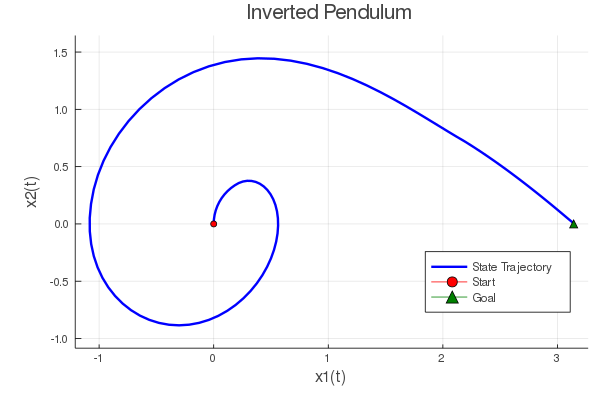
\includegraphics[scale=0.2]{figures/2d_pendulum_spiral}
			\caption{The nominal open-loop trajectory of the $2$-dimensional pendulum.}
			\label{fig:traj 2d pendulum}
		\end{figure}
\end{remark}

Now we present some optimization for Step~\ref{step:abcd} of Alg.~\ref{alg:main} that significantly improved the computation time.

\subsection{Optmization: Local ABCD around the nominal trajectory}\label{sec:local_abcd}
Usually, in ABCD the abstraction process requires computation of abstract transitions all over the state space, which is computationally expensive.
Luckily, for Step~\ref{step:abcd} of Alg.~\ref{alg:main}, we only need to compute transitions in the $\varepsilon$-neighborhood of the given nominal trajectory.
We summarize our optimized approach for Step~\ref{step:abcd} in Algorithm~\ref{alg:abcd-with-time-for-tracking}.
For simpler notation, we omit the robot index $i$.
Given a robot's model as a control system $\Sigma$, together with a reference open-loop trajectory satisfying $\Phi_\varepsilon$ and a tube size $\varepsilon\in \reals_{>0}^n$, we iteratively construct a tube $P$ as union of $\varepsilon$-balls around the reference trajectory's points. 
Next, we compute finite state abstraction for $\Sigma$ setting $Domain=P$ and for the chosen parameters $\eta_x$, $\eta_u$ and $\tau$. 
Finally, Given the computed finite state abstraction $\widehat \Sigma$ and the LTL specification in Eq.~\eqref{eq:ltl_spec}, we synthesize controller using usual ABCD, implemented using SCOTS. %\MS{perhaps we can add a discussion here about our actual implementation.}

We use Alg.~ \ref{alg:abcd-with-time-for-tracking} for solving Prob.~\ref{prob:tracking_with_time} using finite abstraction.
% It means we embedding extra state variable, which represents time. Here we use notation $\Psi_\epsilon(\widetilde{x})$ which is very similar to $\ball_\varepsilon(x)$.
%$\Psi_\epsilon$ denotes the ball radius $\varepsilon$ centered around $X$ and radius zero for time $t$.
%Formally:\\ $\Psi_\epsilon(\widetilde{x}=\begin{bmatrix} x \\t \end{bmatrix}):= \set{\widetilde{x}'=\begin{bmatrix}
%	x' \\
%	t'
%	\end{bmatrix}
%	\in \widetilde{X}\mid  \| x-x' \|\leq \varepsilon \land (t=t')}$\\
%we are using Alg \ref{alg:abcd-with-time-for-tracking} for solving Prob \ref{prob:tracking_with_time} using finite abstraction



%Alg.~\ref{alg:abcd-for-tracking} outlines the steps for solving Prob.~\ref{prob:tracking} using finite state abstraction.

\begin{algorithm}
	\caption{ABCD-for-tracking}
	\label{alg:abcd-with-time-for-tracking}
	\begin{algorithmic}[1]
		\Require $\Sigma=(X,U,W,f,Y,h)$, $\tau \in \mathbb{R}_{>0}$, $\eta_x\in \mathbb{R}^n_{>0}$, $\eta_u\in \mathbb{R}^m_{>0}$, $(x_{0,\nom},\ldots,x_{T,\nom})$, $\varepsilon \in \mathbb{R}_{>0}^{n}$
		\Ensure Feedback controller $C\colon X\times [0;T]\to U$ (partial function)
		\State $P \gets \emptyset$
		\For{$t$ from $0$ to $T$}
		\State $P \gets \ball_{\varepsilon}(x_{t,\nom})$
		\EndFor
		\State $(\widehat{\Sigma},Q) \gets \findAbs(\Sigma, P, \tau, \eta_{x} , \eta_u)$
		\State Synthesize controller $\widehat{C}$ for $\widehat{\Sigma}$ and the specification given in Eq. \eqref{eq:ltl_spec} %$(\ball_{\varepsilon}(x_K^\nom,k), \emptyset, (x_0^\nom,0))$
		\State \Return $\widehat{C}\circ Q$
	\end{algorithmic}
\end{algorithm}

%\subsection{Some ALTRO-specific implementation details}

%In the following, we summarize some ALTRO-specific implementation details.



